%!TEX root = thesis.tex
In the previous chapters we have investigated our initial interpretation of AHIs through inspirational user studies and prototyping.
Our initial thoughts on AHIs were based on existing research directions and inspiration from the domestic domain which led us to the idea of AHIs as a novel interaction approach that, in our optics, touches upon some little explored areas of HCI.  
As we have now gone through three very different approaches to the creation of AHIs it is now time to zoom out from the individual details of the approaches and revisit our concept of AHIs based on our experiences, both the successful and the less successful.

\section{Revisiting the definition of AHIs}
In this section we will revisit our original definition of ad hoc interfaces in the light of the concepts and prototypes that were the results of our three construction approaches that followed the definition.

\subsection{Definition and experiences}
In chapter 4 we defined AHIs as
\begin{quotation}
\emph{Tangible interfaces that can be created or accessed on demand for a particular purpose and with the user as the initiator of action. When in use the interface will temporarily emerge to the foreground after which it disappears into the background, either physically or perceptually.}
\end{quotation}
Here we will address the definition part by part in relation to our experiences from chapters 6--8.

\subsubsection{Created or accessed on demand}
This part of the definition expresses the initial encounter with an AHI.
In our three different explorations we have approached this aspect of the definition in very different ways.
Textile Touch is an example of \emph{accessing} the interface mediated through an existing object.
In our case Textile Touch was implemented as a general purpose touch interface for multiple applications, i.e. the audio and video application.
So, the specific interface for the particular purpose is in a sense created on the spot, for instance the shift between video and audio control.
This does not affect the physical manifestation of the interface as it is a virtually created interface and as such we see it as an accessed interface.

Conductive Paint, on the other hand, is clearly an example of a physically \emph{created} interface.

With the jamming concepts there is not a clear distinction as there are aspects of both created and accessed interfaces.
A more appropriate term would be \emph{adapted} or \emph{formed} interfaces, pointing to an addition to our definition.

\subsubsection{The user as the initiator} 
Again we see different interpretations of the definition.
Textile Touch takes a traditional approach where the user explicitly initiates some action or activity.
Jamming and Conductive Paint are more interesting in this regard.
In Conductive Paint the initiation of action refers to the actual creation of the interface as this is the part where the purpose of future interaction is being defined.
In some of the jamming concepts (Improvised Furniture and Playful Blobs) the user initiates the action by shaping the interface for a particular purpose.
So generally we see the user as the initiator of action though the action has different purposes in the different examples.

\subsubsection{Foreground and background}
Foreground refers to the center of action and as all our prototypes have a degree of direct interaction the interpretation of foreground does not vary much between the approaches.
However, the transition from foreground to background is more loosely interpreted as to how the interface should \emph{disappear} into the background.
As Textile Touch does not have a physical manifestation, other than the object that it embeds itself in, the notion of background is more of a perceptual character.
So the interface disappears but in a more virtual than physical way.
The only physical traits that disappear are the haptic and visual feedback from the interface.

The transition from foreground to background in Conductive Paint can be seen in two different way.
In one sense the interface will fade into the background when not in use by being just an artistic expression on the wall, so more of a passive perceptual transition.
The other aspect is the true disappearance of the interface when it is removed.
As we envision this a an interface that can equally easy be constructed as removed, this transition is a very concrete interpretation of the disappearance.

Lastly in our jamming concepts, and BeoMotion, we see the disappearance into the background as the interface deforming itself into a natural state, which is a mix between a physical and perceptual disappearance.  

A note is that we see a general tendency for the interfaces to be relevant while in the background, in the sense that they have an intrinsic meaning while not in use.
At least this is the case in Textile Touch, Conductive Paint, Improvised Furniture and BeoMotion and to a less extend Dynamic Input Control.
We see this as an important point because if the interface is not inherently relevant in its background state, in the sense of having a ``natural'' or ``passive'' function, it is less likely that the interface perceptually enters this background state, in the eyes of the user.
So the transition from foreground to background also points to a transition between an active and a passive function, where passive functions could be aesthetic, as in Conductive Paint, or inherited from the object that has been embedded, as in Textile Touch and BeoMotion.

\subsubsection{Interfaces that disappear}
\citet{abowd2012next} notes that, while many of Weiser's predications about the future of computing have come true, some were not so accurate such as inch-scaled devices being readily disposable.
While this is true, our concept of AHIs does, in some aspects, challenges this as we propose that AHIs \emph{disappear} after use.
We see this disappearance both in the sense of the affordance or perception of the interface, so here not a physical disposal in the sense that \citeauthor{abowd2012next} is referring to, but also in the sense of the physical removal of the interface.
This is apparent in Conductive Paint as we here suggest that interfaces are built on the spot which will, at least in some cases, also lead to deconstruction of the interface after use and therefore be disposable in the sense \citeauthor{abowd2012next} is referring to.

As we saw with our exploration of paint as a construction mechanism the interface could be disposed simply with a wet cloth.
From a sustainability point of view disposable interfaces are of course not an unproblematic approach.
So a future focus for such interfaces should be to focus on reuse.
In our paint interface this could for example mean that the paint is collected in a container for later re-use instead of simply being washed away. 

\subsection{A possible fourth approach}
In our exploratory evaluation of Textile Touch we saw a pointer to a way of approaching AHIs that we had not considered in our initial outline of the concept.

Where we with the Textile Touch prototype have focused on it as an example of how interaction can be integrated into the existing environment in a ubiquitous fashion, it can also be used as an example of how to extend the capabilities of existing objects and to augment their functions in an ad hoc manner.

At a glance this does sound somewhat like Augmented Reality (AR), but as \citet{azuma1997survey} describe AR it \emph{allows the user to see the real world, with virtual objects superimposed upon or composited with the real world.}
So the focus is on augmenting the environment \emph{virtually}, while our proposed focus is on augmenting the environment \emph{physically}.

Inspired by this idea of augmenting existing objects in an ad hoc fashion, we have taken a brief look around for other examples that might give weight to this approach.

REVEL \citep{bau2013revel}, as we have briefly mentioned earlier, is a system that via a digital overlay augments objects by changing the tactile perception of their physical surface.
So it is a physical augmentation that, in principle, can be done to arbitrary objects giving them a new physical sensations while retaining the existing properties of the object.

Another example is Pinoky \citep{sugiura2012pinoky} that is a wireless ring-like device that can augment ordinary plush toys to allow them to move limbs.
This is done by attaching the ring around a limb to actuate it and the Pinoky can now record movements done by the user and play them back, animating the plush toy.

Common for both these examples is the ad hoc augmentation of non-interactable objects (in an computing sense), changing their inherent physical properties, as in REVEL, or giving them new interactable properties, as in Pinoky.

We see this as an interesting aspect of future AHIs and a direction that should be explored more in depth, both in terms of more precise definition of the approach and in terms of an actual exploration through literature, concepts and prototypes.

\subsection{A modified definition}
As we have now analysed the different aspects of our initial definition of AHIs in relation to our concepts and prototypes we present a modified version of the definition of AHIs.
We now define AHIs as
\begin{quotation}
\emph{Tangible interfaces that can be created, adapted or accessed on demand for a particular purpose and with the user as the initiator of action. In use the interface will emerge, either physically or perceptually, to the foreground and transition into a meaningful background state when inactive.}
\end{quotation}

Along with this definition we now argue for four approaches to the creation of such interfaces,

\begin{itemize}
	\item{Using shape change as the construction mechanism.}
	\item{Through invisible interfaces embedded into the physical environment.}
	\item{Literally constructing the interface on the spot.}
	\item{Augmenting existing objects or interface dynamically.}
\end{itemize} 

\section{Understanding interaction with AHIs}
\begin{quotation}
\emph{When Koffka asserted that ``each thing says what it is'' he failed to mention that it may lie. More exactly, a thing may not look like what it is \citep{gibson1979ecological}.}
\end{quotation}
The above quote from \citeauthor{gibson1979ecological} is especially interesting in relation to AHIs as it points to a challenge that we have not really touched upon in this thesis.
As AHIs have an inherently dynamic nature, how do we ``pick up'' the interaction possibilities of the interface? 
In the following we will take a look at our experiences with AHIs in the light of affordance theories to assert whether affordances can help to communicate intent in such dynamic interfaces as AHIs and point to possible areas of improvement.

\subsubsection{Affordances}
The notion of affordances describes the relationship between the acting organism and the acted-upon environment.
The term comes from the above cited perceptual psychologist J.J. Gibson.
Affordances are properties of the environment that, for good or bad, tells us about the possible actions that are available to us.
Affordances therefore describe the potential for actions in the environment as we perceive that environment.  

\subsubsection{Perception and Affordances}
Perception is a key concept in relation to affordances as in order to ``know'' an affordance is there, you have to perceive it with your senses. Where \citet{gibson1979ecological} focuses mostly on visual perception, \citet{gaver1991technology} wants to broaden it to include all the senses, such as tactile and auditory feedback.
For example, sound can be used to indicate affordances that cannot be seen, where the sound of a turning lock indicates that the affordance of the door has changed.

\citet{gaver1991technology} notes that \emph{``Affordances per se are independent of perception''}.
This separation of affordances and the information available about them to us, gives rise to complications, as affordances will still exist even if you do not perceive them or if you perceive them wrong.
Additionally, you might perceive an affordance that does not exist.

This leads back to the opening quotation from Gibson as there, in the case of AHIs, is a possibility that an object does not have perceivable affordances that match the actual affordances.
If we look at our first AHI construction approach that we suggested in chapter~\ref{ch:adhoc}, we proposed an approach where objects change their shape.
Dynamic shapes would allow for dynamic, or changing, affordances where the perceived action possibilities of an object would change based on the change in shape.
So one form-instance of a dynamic object does not necessarily allow for the perceptibility of all the possible affordances of that object, leading to, in Gaver's term, hidden affordances. 
The same is true for our embedded invisible interfaces where the perceived affordances will most likely be tied to the object in which the interface is embedded and not the interface itself.

So Gibson's focus on what can be \emph{seen} does not fit dynamic objects.
Gaver suggests a more exploratory approach for interfaces with complex affordances, which is where AHIs fit, where the affordances are learned through their use and interaction.
The notion of learning through use is especially relevant for Textile Touch as we envision it as an interface that should, over time, provide effortless interaction which only requires peripheral attention.

The exploratory approach is taken up by \citet{djajadiningrat2004tangible} who suggest a focus on both appearance and action as carriers of meaning.

\subsubsection{Appearance and Action}
Another way to approach the question about how objects appeal to our senses and motor skills is presented by \citet{djajadiningrat2004tangible}.
As we have seen above traditional focus of affordance concerns appearance and action, where affordances invite an arbitrary action. 
In this sense it is the appearance, both visual and physical, of an object that carries the meaning.

\citeauthor{djajadiningrat2004tangible} argue for an approach where the focus is on \emph{both} appearance and action as carriers of meaning, inextricably linking usability and aesthetics.
In this way action and appearance both express something about the purpose of the interface and they identify two options for creating meaning through this expressiveness, a semantic and a direct.

In the \emph{semantic} approach meaning is derived from semantics and cognition.
So metaphors, for example, can trigger associations to other products or concepts with which the user is familiar.
This approach is somewhat in play in Textile Touch as the interaction should, ideally, draw on the common touch interaction patterns that are prevalent in today's smart phones and tablets.
In retrospect this should have had more focus in our test application for Textile Touch as some of our patterns were too disconnected from the action they performed creating a mismatch between the expected outcome and the actual outcome.
Further work on this could with advantage refer to \citep{wobbrock2009user,morris2010understanding} for an understanding of gestures and user generated gestures.

In the \emph{direct} approach meaning is created in the interaction with physical objects and therefore there is a strong emphasis on the perceptual and bodily skills of the user.
The idea is that meaning is created in interaction, much resembling Gaver's `learning through use'. 
This could be one way to understand shape changing AHIs as their action possibilities shift with changes in form, especially if the user is the manipulator of form.
One thing we noticed when experimenting with shape change, both in chapter~\ref{ch:workshops} and \ref{ch:jamming}, was that it was quite hard to agree on forms when the interface had many degrees of freedom.
So given a ``blob'' that could deform in any way, in our case a piece of plasticine, we saw difficulties in continuously recreating the same forms, which would be needed for a direct mapping between form and function.
This is problematic as it would make it hard to ``learn'' the interface if forms are hard to consistently match.
So in order to create meaning in interaction for such interfaces we see the need for constraints to the number of possible forms that can be made, in that way retaining the physical exploration but in a limited fashion.

Interestingly \citet{lee2010users} has made a study on the physical deformation and the related action that the deformation maps to, and find that the agreement on the mapping \emph{increases} with higher degrees of freedom, which seems counter-intuitive.
Whether this finding can be transferred to 3D objects, which are inherently more complex than paper, would be interesting to test in a more thorough setting than ours.
While we do not anticipate that it would be true for a free-form object, perhaps a middle ground exists between a certain amount of form constraints and form freedom that proves to give a more effective mapping between form and function.
\blank
Our conductive paint exploration from chapter~\ref{ch:prototype3} is quite different from the other two approach in terms of affordances.
As it is up to the user to construct the interface there is no initial perceptual or tangible guidelines to direct interaction or construction. Though the interesting aspect of our example of painting the wires and switches on the walls, is that it creates a, in Norman's terms \citep{norman2002design}, \emph{natural mapping} between the interface control and the controlled object as there would be a direct visual link between the two.
If this would lead to natural interaction is only speculative but it does point to a possible quality of such interfaces. 

\subsubsection{Feedback and Feedforward}
We have already covered the aspect of affordances previously in this chapter as a way to discuss and inform our prototypes and concepts.
Here we will look at an approach that we believe future AHIs could benefit from in order to increase the user experience and understanding of the interface and its functions.

The Interaction Frogger is a framework \citep{stienstra2012design,wensveen2004interaction} that gives us tools to understand and improve designs in relation to the coupling between user actions and the product's functions through the use of feedback and feedforward.

While feedback is the repose that a user gets from an action, feedforward is seen as the mechanism that invites a user to action and therefore happens before the user's action takes place. 
Three types of feedforward are identified; \emph{inherent, functional and augmented}, along with six aspects of action-function coupling; \emph{time, location, direction, dynamics and modality}.
This makes up the different parts of the interaction loop that can be used to analyse and augment the interaction.

The idea of feedforward is especially intriguing in relation to AHIs that make use of shape-change.
If we see interaction as a continuous action-perception loop, an interface with a dynamic form could potentially influence the user's interpretation of the action possibilities by continuously changing its shape, as a method of providing feedforward.
This would change both the inherent feedforward of the interface but possibly also serve to augment the feedforward through the transition phase.
So there are feedforward capabilities in both the end-shape and in the transitions between shapes in such dynamic interfaces.
This type of dynamic feedforward could be a possible approach to help reveal the form possibilities of dynamic interface and their associated functions.

Generally we see the Interaction Frogger framework as an interesting tool in relation to dynamic interfaces as to improve the user's understanding of interfaces that changes form or function.
We expect great benefit from exploiting this framework for future work on AHIs to address the difficult challenge of perceiving hidden and embedded action affordance.

%As we have already touched upon feedback in the prototyping chapters, we will limit ourselves to discuss feedforward here.
%Inherent feedforward is related to the perceptual action possibilities of an interface, in this sense much in line with Gibson's \citep{gibson1979ecological} view on affordances.
%Functional feedforward informs about the general purpose of an interface, for example through semantics or visibility of functional parts.
%Augmented feedforward is when the user receives information about the action possibilities from an additional source, such as words or sounds. 

\subsubsection{A taxonomy for tangibles}
The last topic we will cover in this section is a look into Fishkin's taxonomy for tangible interfaces \citep{fishkin2004taxonomy}.
The taxonomy uses two axes, \emph{metaphor} and \emph{embodiment} to address how `tangible' an interface is.
\emph{Embodiment} describes the relationship between the input focus and the output focus, while \emph{metaphor} describes the level of metaphorical ties the interface has, that is the level of a real-world analogy the interface has.

So can we, based on our prototypes and concepts, say something general about AHIs in terms of this taxonomy?
In figure~\ref{fig:ch:adhoc2:fishkin} we have placed our various AHIs to give an overview and look for eventual tendencies. 

\begin{figure}[h]
  \centering
  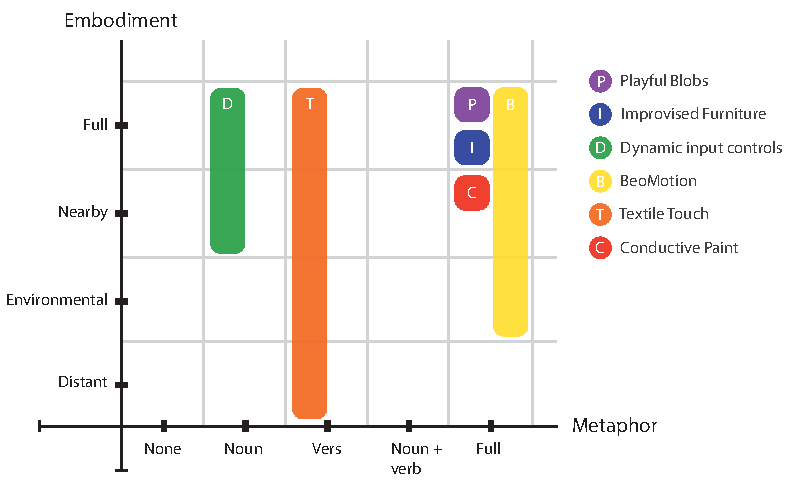
\includegraphics[width=.9\textwidth]{figures/adhoc2/fishkin.pdf}
  \caption[Placements of our prototypes and concepts in Fishkins taxonomi]
  {Placements of our prototypes and concepts in Fishkins taxonomi for tangible interfaces.}
  \label{fig:ch:adhoc2:fishkin}
\end{figure}

While it was more or less straight-forward to place the different prototypes and concepts on the scale of embodiment, it was a lot less given on the scale of metaphor.
As can be seen there is a tendency for a high degree of embodiment.
In Textile Touch we find that it depends quite a lot on the use situation as to how embodied the interface is.
While we envision situations and applications where the feedback and content is on the Textile Touch surface, where there would be a high degree of embodiment, other applications, such as controlling appliances in the near surrounding would have a lesser degree of embodiment.
The AHIs that involve shape-change generally show a high degree of embodiment when change of shape is used for both input and output.

The placements on the metaphor axis are less certain.
One of the challenges here is that Fishkin focuses on real-world analogies.
So in our Playful Blobs for example we actually use digital-world analogies, such as \emph{copy/paste}, \emph{save} and \emph{open}, to describe real-world interaction.
So either we have \emph{no} metaphor, as there is no real-world analogy, or we bend the taxonomy a little and use \emph{verb} and accept the digital-world analogy for our tangible interface, or lastly we could see it as a \emph{full} metaphor as the virtual system \emph{is} the
physical system. 
We have placed it as a full metaphor as we argue that we have truly direct manipulation in the interface, merging the physical and digital system.

Generally we do see a high degree of tangibility in AHIs, at least based on our interpretation of the taxonomy, which does fit our goal of such interfaces as we seek to tie the physical and digital aspects of interfaces closer together, drawing on the qualities of both worlds.
The individual placements can of course be discussed as some of the examples could possibly have a different placement, but we do see a tendency in AHIs towards \emph{more tangibility} rather than less tangibility. 
